\section{Boni}
Ce chapitre contient des bonus. Vous serez moins guidées, et des vous aurez des
liens vers les pages de documentation pour vous aider à avancer.

En réalisant ces boni, vous pourrez arriver à un résultat proche de celui-ci :
\begin{center}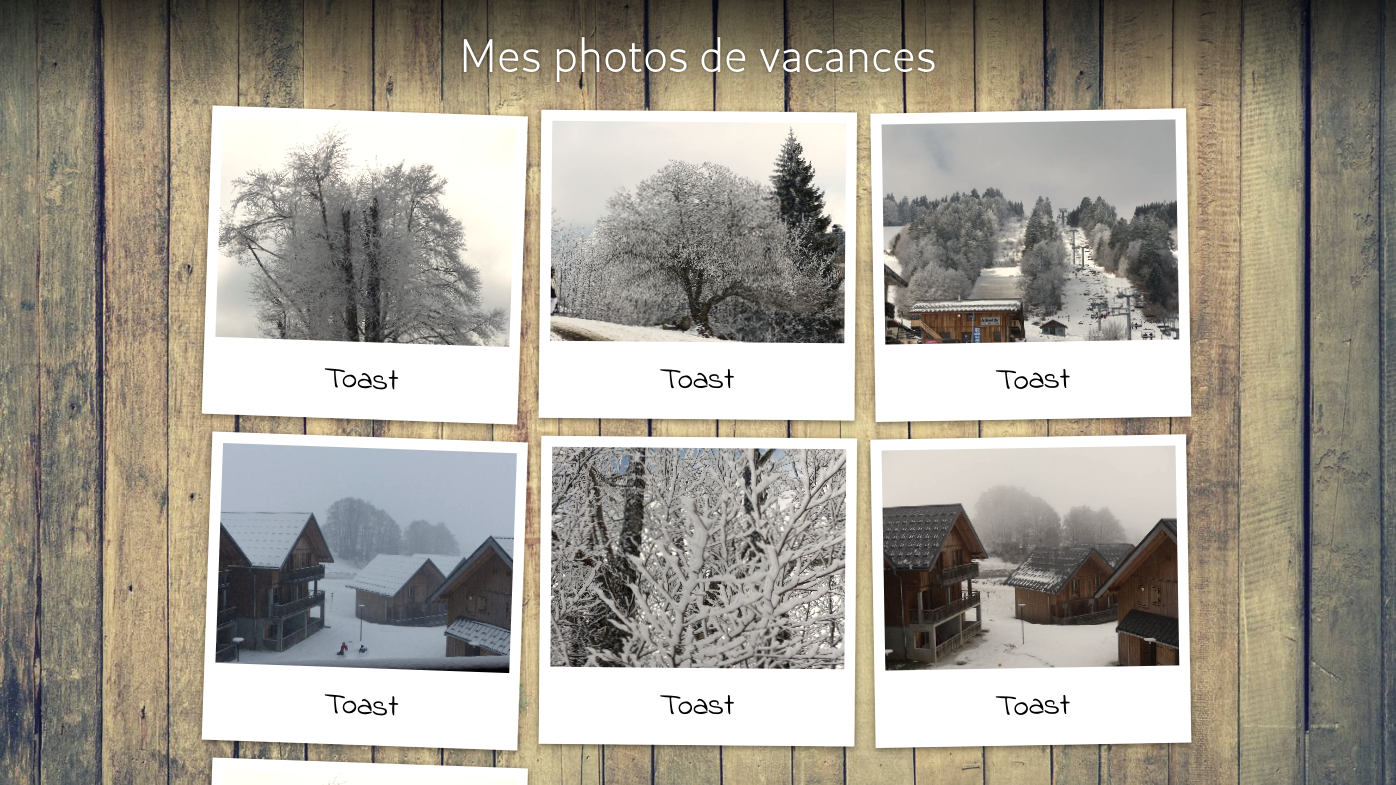
\includegraphics[width=.8\linewidth]{img/screenshot_final.png}\end{center}

\subsection{Une police d'écriture plus sympathique}
Grâce à la propriété CSS font-family il est possible de définir une autre police
d'écriture que celle par défaut.
\subsubsection{Cantarell}
Dans ma solution j'utilise la police Cantarell, qui est une généralement
disponible sous Linux. Cependant la majorité des gens n'utilisent pas Linux, et
je vous recommande donc d'utiliser une police disponible sur \href{https://fonts.google.com}{Google Fonts}.

Ici, j'ai utilisé "Cantarell Thin" pour la balise h1 du header, et "Cantarell"
pour le footer.
\subsubsection{Besoin de plus de polices ?}
Grâce au site \href{https://fonts.google.com}{Google Fonts}, vous pouvez trouver
plus de polices à utiliser dans votre site.

\begin{center}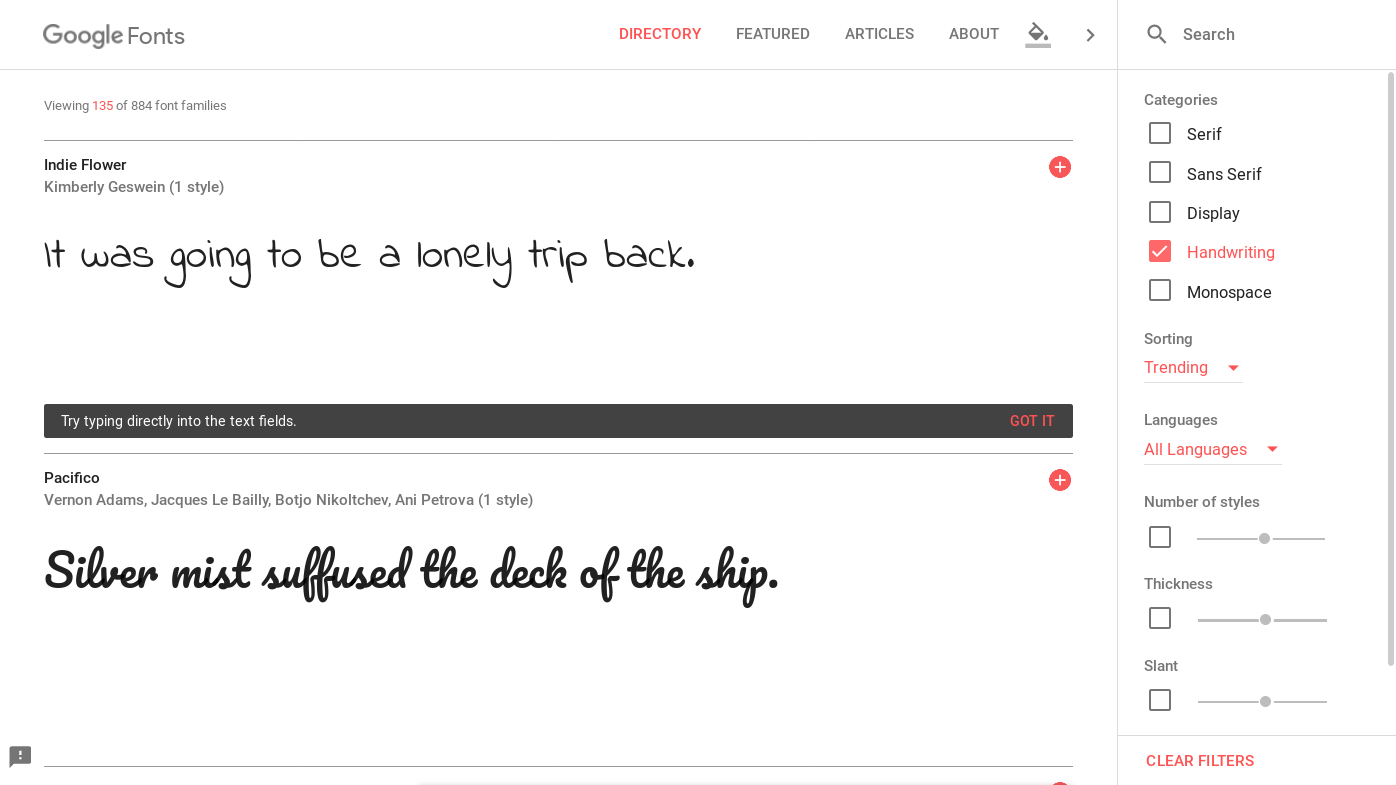
\includegraphics[width=.8\linewidth]{img/screenshot_google_fonts.png}\end{center}

Comme vous pouvez le voir dans cette capture d'écran, Indie Flower, la police
utilisée par les éléments figcaption dans la solution, est la première de la
catégorie "Handwriting" (écriture à la main).

Pour utiliser la police, vous devrez cliquer sur le (+) en haut à droite de la
police, puis en bas de la page cliquer sur le bloc noir avec écrit
"1 famille sélectionnée".

Une fois le bloc déroulé, vous verrez une balise HTML à ajouter dans la balise
head de votre page, et aussi une ligne de CSS vous montrant comment l'utiliser.

\subsection{Les ombres portées}
Afin de donner un peu plus de relief à notre site, nous pouvons rajouter des
ombres sous différents éléments. Pour cela, l'attribut css box-shadow est notre
sauveur.

Nous allons ici utiliser la représentation RGBA des couleurs pour son avantage
principal : la transparence. Vous pourrez ainsi créer une ombre moins "franche"
qu'avec un code hexadécimal. Par exemple pour faire un noir opaque à 70\%, la
couleur s'écrit rgba(0,0,0,0.7)


Dans la solution finale, j'utilise des box-shadow sur les figure et le footer.

Sa documentation se trouve \href{https://developer.mozilla.org/fr/docs/Web/CSS/box-shadow}{ici}.

\subsection{Une rotation "aléatoire"}
Pour faire cette effet j'utilise tout d'abord le sélecteur CSS nth-child, puis
j'applique une rotation avec la propriété transform.

J'utilise le sélecteur nth-child pour appliquer une rotation à un élément sur
trois, puis une autre à un élément sur trois plus un...

La documentation de transform se trouve \href{https://developer.mozilla.org/fr/docs/Web/CSS/transform}{ici}.
La documentation pour nth-child se trouve \href{https://developer.mozilla.org/fr/docs/Web/CSS/:nth-child}{ici}

\subsection{Un filtre sépia sur  les photos}
Avec la propriété CSS "filter", il est possible d'ajouter des filtres à des
éléments.

Ici, j'utilise le filtre sepia à 20\% sur les photos lorsqu'elles ne
sont pas survolées

Sa documentation se trouve \href{https://developer.mozilla.org/fr/docs/Web/CSS/filter#sepia()_2}{ici}.

\subsection{Les grilles CSS}
Les grilles CSS sont une technologie très récentes, moins d'un an, mais elles
permettent de créer des designs web complexes assez rapidement.

Pour voir ce que permettent les grilles CSS, vous pouvez regarder
\href{https://labs.jensimmons.com/}{le site de Jen Simmons}, développeuse et
designer web travaillant à Mozilla.

Les grilles permettent d'organiser la page en fonction d'une grille, dont vous
pouvez changer la taille des cases, l'espacement entre les cases etc...

Un petit cours d'anglais : une ligne se dit "row", une colonne "column", et un
espacement "gap".

La documentation des grilles se trouve \href{https://developer.mozilla.org/fr/docs/Web/CSS/CSS_Grid_Layout#CSS}{ici}.

\subsubsection{Une grille par photo}
\begin{center}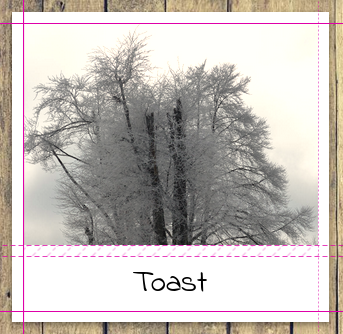
\includegraphics[width=.5\linewidth]{img/grid_figure.png}\end{center}
Ici, j'ai appliqué une grille de deux lignes avec grid-template-rows, où la
première fais 4fr la seconde 1fr, et le grid-row-gap est de 10px.

\subsubsection{La grille principale}
Ici, la grille est définie avec
\begin{minted}{css}
grid-template-columns: repeat(auto-fit, minmax(270px, 1fr));
\end{minted}
Cela permet de faire en sorte qu'il y ait autant de photos que possible, mais
qu'elles fasse au minimum 270px de large.

Aussi, j'applique un grid-gap de 16px pour espacer les photos entre elles.


\subsection{Fin}
Félicitations ! Il reste encore certains morceaux de la solution qui ne sont pas
faisables juste en suivant ce TP, si vous le souhaitez vous pouvez regarder la
solution, et essayer de comprendre ce qui n'est pas expliqué ici en utilisation
la documentation MDN.
